\documentclass{article}

%other packages
\usepackage[a4paper]{geometry}
\usepackage{longtable}
\usepackage{wrapfig}
\setlength\parindent{0pt}
\usepackage{enumitem}
\usepackage[table,dvipsnames]{xcolor}
\usepackage{polynom}
\def\scaleint#1{\vcenter{\hbox{\scaleto[3ex]{\displaystyle\int}{#1}}}}
\usepackage{array}
\newcolumntype{C}{>{{}}c<{{}}} % for '+' and '-' symbols
\newcolumntype{R}{>{\displaystyle}r} % automatic display-style math mode 
\usepackage{tabularray}
\usepackage{dcolumn,tabularx,booktabs}
\usepackage[most]{tcolorbox}

%maths
\usepackage{mathtools}
\usepackage{amsmath}
\usepackage{amssymb}
\usepackage{amsfonts}
\usepackage{autobreak}

%tikzpicture
\usepackage{tikz}
\usepackage{scalerel}
\usepackage{pict2e}
\usepackage{tkz-euclide}
\usepackage{tikz-3dplot}
\usetikzlibrary{calc}
\usetikzlibrary{patterns,arrows.meta}
\usetikzlibrary{shadows}
\usetikzlibrary{external}
\usetikzlibrary{decorations.pathreplacing,angles,quotes}

%pgfplots
\usepackage{pgfplots}
\pgfplotsset{compat=1.18}
\usepgfplotslibrary{statistics}
\usepgfplotslibrary{fillbetween}

\pgfplotsset{
    standard/.style={
    axis line style = thick,
    trig format=deg,
    enlargelimits,
    axis x line=middle,
    axis y line=middle,
    enlarge x limits=0.15,
    enlarge y limits=0.15,
    every axis x label/.style={at={(current axis.right of origin)},anchor=north west},
    every axis y label/.style={at={(current axis.above origin)},anchor=south east}
    }
}

\begin{document}

Jaglal, Tyler - Math 115 AS01 - Typesetting Portfolio
\hrule

\vspace{10pt}

This is the 3D Cartesian graph of the function $\displaystyle f(x,y)=\frac{\sin(\sqrt{x^2+y^2})}{\sqrt{x^2+y^2}}$ (credit for code: the pgfplots manual)

\begin{center}
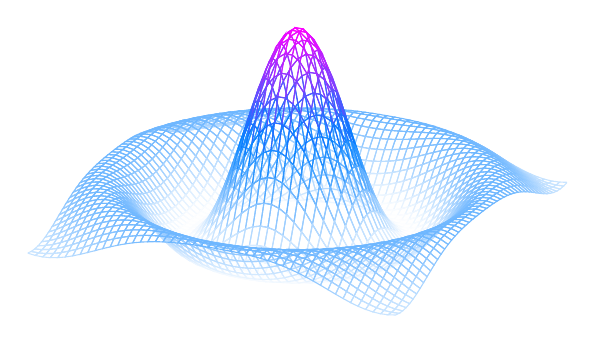
\begin{tikzpicture}
\begin{axis}[colormap/cool, hide axis,
mesh,
    samples=50,
    domain=-8:8,]
\addplot3[mesh, samples=50]{sin(deg(sqrt(x^2+y^2)))/sqrt(x^2+y^2)};
\end{axis}
\end{tikzpicture}
\end{center}

This is the surface area of revolution of the function $y=2^x$, about the $x$-axis: (of my own creation)

\begin{center}
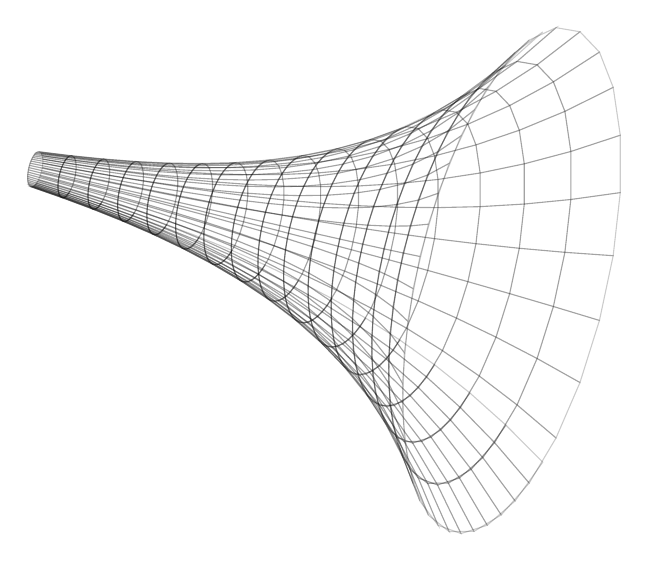
\begin{tikzpicture}[scale=1]
\begin{axis}[
hide axis,
view={25}{30},
scale=3,
unit vector ratio=2 1 1,
]
\addplot3[
mesh,
color=black,
opacity=0.2,
samples=40,
restrict x to domain=-2:2,
]({x},{(2^x)*cos(deg(y))},{(2^x)*sin(deg(y))});
\end{axis}
\end{tikzpicture}
\end{center}

This is a 3D graph of the funtion $y=1+\frac{1}{5}\sin(5\phi)\sin(6\theta)$ in spherical coordinates: (credit for formula: Stewart, otherwise of my own creation)

\begin{center}
\tdplotsetmaincoords{60}{110}
\begin{tikzpicture}[scale=2,line join=bevel,tdplot_main_coords,%
fill opacity=.5]
\tdplotsetpolarplotrange{0}{360}{0}{360}
\tdplotsphericalsurfaceplot[parametricfill]{72}{36}%
{1+(1/5)*sin(6*\tdplottheta)*sin(5*\tdplotphi)}{black}{\tdplotphi}%
{\path[color=black,thick,->] (0,0,0)
-- (1,0,0) node[anchor=north east]{};}%
{\path[color=black,thick,->] (0,0,0)
-- (0,1,0) node[anchor=north west]{};}%
{\path[color=black,thick,->] (0,0,0)
-- (0,0,1) node[anchor=south]{};}%
\end{tikzpicture}
\end{center}

\newpage

This is a slope field representing the differential equation $y^\prime=2x+y$: (of my own creation)

\begin{center}
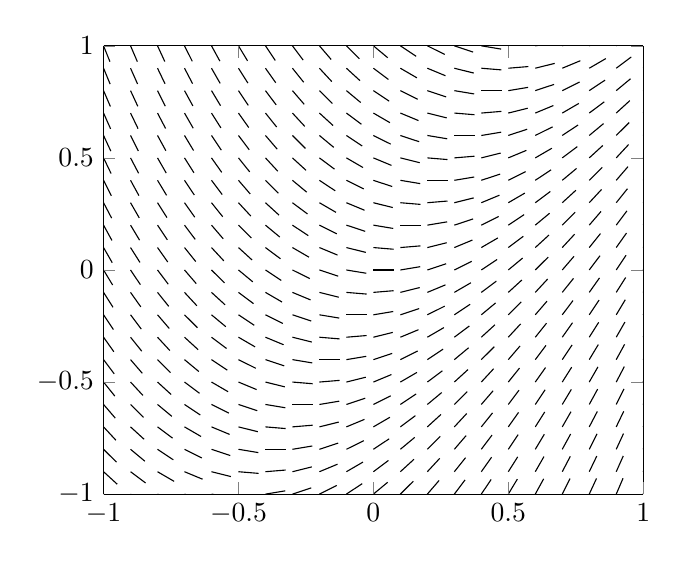
\begin{tikzpicture}
\begin{axis}[
    view={0}{90},
    domain=-1:1,
    y domain=-1:1,
    xmax=1, ymax=1, ymin=-1,
    zmin=-1, zmax=1,
    samples=21
]
\addplot3 [quiver={u={1/(sqrt(1+(2*x-y)^2))}, v={(2*x-y)/(sqrt(1+(2*x-y)^2))}, scale arrows=0.075, every arrow/.append style={-}}] (x,y,0);
\end{axis}
\end{tikzpicture}
\end{center}

This is a geometric diagram from yesterday's class: (credit: you)

\begin{center}
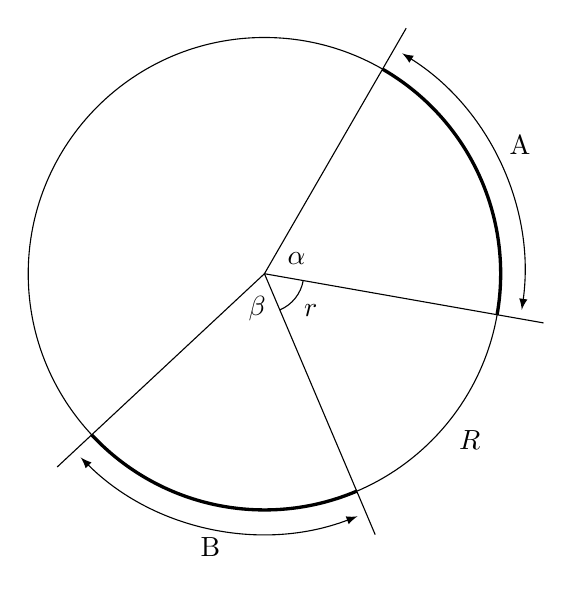
\begin{tikzpicture}[scale=3]
\coordinate (O) at (0,0);
\coordinate (C1) at (-10:1.2);
\coordinate (C2) at (60:1.2);
\coordinate (C3) at (223:1.2);
\coordinate (C4) at (293:1.2);
\draw[] (O) circle [radius=1];
\draw[] (C1) -- (O) -- (C2);
\draw[] (C3) -- (O) -- (C4);
\draw pic["$\alpha$",angle eccentricity=1.5, angle radius=0.3cm]{angle=C1--O--C2};
\draw pic["$\beta$",angle eccentricity=1.5, angle radius=0.3cm]{angle=C3--O--C4};
\draw pic["$r$",draw,-,angle eccentricity=1.5, angle radius=0.5cm]{angle=C4--O--C1};
\draw[very thick] (-10:1) arc [start angle=-10, end angle=60, radius=1];
\draw[latex-latex] (-8:1.1) arc [start angle=-8, end angle=58, radius=1.1] node[pos=0.5,above right]{$\mathrm{A}$};
\draw[very thick] (223:1) arc [start angle=223, end angle=293, radius=1];
\draw[latex-latex] (225:1.1) arc [start angle=225, end angle=291, radius=1.1] node[pos=0.5,below]{$\mathrm{B}$};
\path[] (293:1) arc [start angle=293, end angle=350, radius=1] node[pos=0.5,below right]{$R$};
\end{tikzpicture}
\end{center}

\newpage

This is the $\angle30^\circ-60^\circ$ triangle. We can reflect it to obtain an equilateral (or ``regular") triangle - something which we know the dimensions of, and which allows us to easily find the sidelengths of our special triangle using Pythagoras's Theorem: (credit: you)

\begin{center}
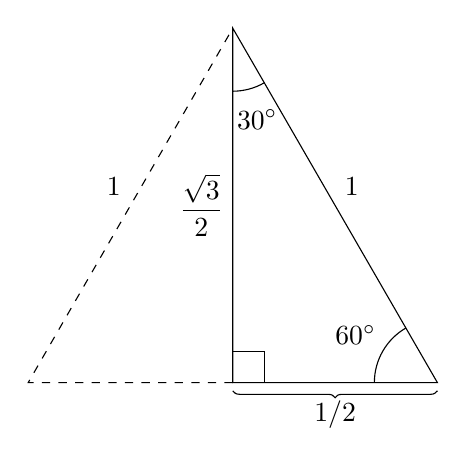
\begin{tikzpicture}[scale=3]
\coordinate (A) at (-30:1);
\coordinate (B) at (90:1);
\coordinate (C) at (210:1);
\coordinate (M) at (210:1 -| 0,0);
\draw[] (M) -- node[pos=0.5,left]{$\displaystyle\frac{\sqrt{3}}{2}$} (B) -- node[pos=0.5,above right]{$1$} (A) -- (M) -- cycle;
\draw[dashed] (M) -- (C) -- node[pos=0.5,above left]{$1$} (B);
\draw pic["",draw,angle eccentricity=1.5, angle radius=0.4cm]{right angle=A--M--B};
\draw pic["$30^\circ$",draw,angle eccentricity=1.5, angle radius=0.8cm]{angle=M--B--A};
\draw pic["$60^\circ$",draw,angle eccentricity=1.5, angle radius=0.8cm]{angle=B--A--M};
\draw [decorate, decoration = {brace,mirror,raise=3pt}] (M) --  (A) node[pos=0.5,below=3pt]{$1/2$};
\end{tikzpicture}
\end{center}

The $45^\circ$ right triangle (which is called an "Isosceles Triangle") is easier to do this with because we can readily apply the Pythagorean Theorem: (credit: you)

\begin{center}
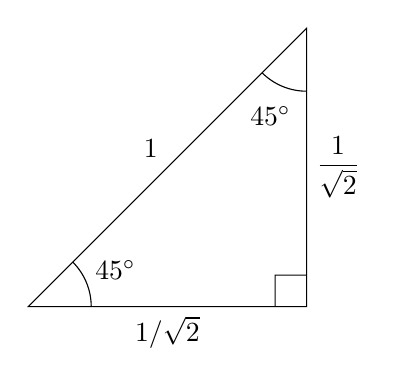
\begin{tikzpicture}[scale=5]
\coordinate (O) at (0,0);
\coordinate (P) at (45:1);
\coordinate (X) at (P |- O);
\draw[] (O) -- node[pos=0.5,above left]{$1$} (P) -- node[pos=0.5,right]{$\displaystyle\frac{1}{\sqrt{2}}$} (X) -- node[pos=0.5,below]{$1/\sqrt{2}$} (O) -- cycle;
\draw pic["",draw,angle eccentricity=1.5, angle radius=0.4cm]{right angle=P--X--O};
\draw pic["$45^\circ$",draw,angle eccentricity=1.5, angle radius=0.8cm]{angle=X--O--P};
\draw pic["$45^\circ$",draw,angle eccentricity=1.5, angle radius=0.8cm]{angle=O--P--X};
\end{tikzpicture}
\end{center}

\newpage

This is a geometric demonstration (from classs) of sine being an odd function, and cosine being an even function: (credit: you)

\begin{center}
\begin{tikzpicture}[scale=3]
\draw[thick,-stealth] (0,-1.3) -- (0,1.3);
\draw[thick,-stealth] (-1.3,0) -- (1.3,0);
\coordinate (O) at (0,0);
\coordinate (P1) at (130:1);
\coordinate (P2) at (-130:1);
\coordinate (X) at (P1 |- O);
\draw[-latex] (0.6,0) arc [start angle=0, end angle=130, radius=0.6] node[pos=0.35,above right]{$\alpha$};
\draw[-latex] (0.6,0) arc [start angle=0, end angle=-130, radius=0.6] node[pos=0.35,below right]{$-\alpha$};
\draw[] (O) -- (P1);
\draw[] (O) -- (P2);
\draw[very thick] (X) -- (O);
\draw [decorate, decoration = {brace,raise=3pt}] (X) -- (O) node[pos=0.5,above=3pt]{$\cos\textnormal{(both)}$};
\draw[dashed] (P1) -- (P2);
\draw[] (P2) -- (0,-0.76604) node[below,pos=0.5]{$\sin-\alpha$};
\draw[] (P1) -- (0,0.76604) node[above,pos=0.5]{$\sin\alpha$};
\end{tikzpicture}
\end{center}

I can also do polynomial long division emaculately (I developed my own style which in my opinion is more consistent and professional looking than the ones in Stewart's review of algebra): (formula from Stewart, but style is my own)

\[\setlength\arraycolsep{0pt} 
\setlength\extrarowheight{2pt}
\begin{array}[t]{ RCCRCRCRCR }
	& & x^2 & - & x & - & 6 & & &\\
\cline{2-9}
	x-2 & \kern-0.4pt\raisebox{1.6pt}{\big)} & x^3 & - & 3x^2 & - & 4x & + & 12 \\
	& & x^3 & - & 2x^2 & & & & & \\
\cline{3-7}
	& & & - & x^2 & - & 4x & & & \\
	& & & - & x^2 & + & 2x & & & \\
\cline{4-9}
	& & & & & - & 6x & + & 12 & \\
	& & & & & - & 6x & + & 12 & \\
\cline{6-10}
	& & & & & & & & 0 &
\end{array}\]

\newpage

This is a diagram that a challenge problem in Stewart has you draw: (credit for formula: Stewart, rest is mine)

\begin{center}
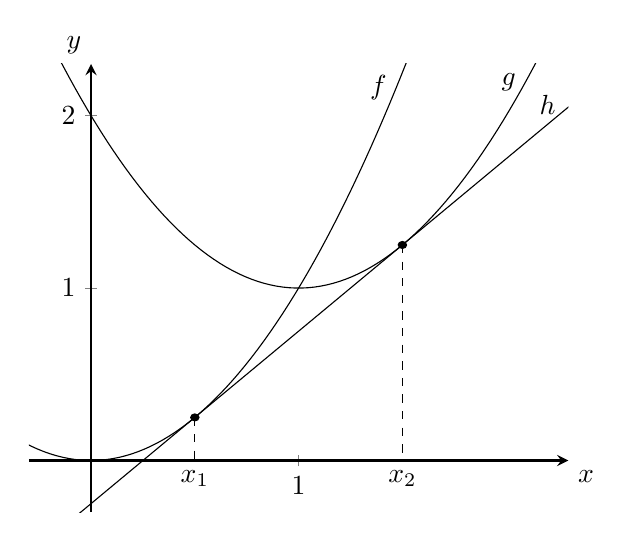
\begin{tikzpicture}
\begin{axis}[
standard,
xmin=0, xmax=2,
ymin=0, ymax=2,
samples=100,
xtick={1},
ytick={1,2},
xlabel={$x$},
ylabel={$y$},
]
\addplot[domain=-0.5:2.5]{x^2} node[pos=0.44, left]{$f$};
\addplot[domain=-0.5:2.5]{(x-1)^2+1} node[pos=0.8, left]{$g$};
\addplot[domain=-0.5:2.5]{x-(1/4)} node[pos=0.9, above]{$h$};
\draw[fill] ({1/2},{1/4}) circle [radius=0.02];
\draw[dashed] ({1/2},{1/4}) -- ({1/2},0) node[below]{$x_1$};
\draw[fill] ({3/2},{5/4}) circle [radius=0.02];
\draw[dashed] ({3/2},{5/4}) -- ({3/2},0) node[below]{$x_2$};
\end{axis}
\end{tikzpicture}
\end{center}

Early on in Stewart we prove the limit of sine x over x equals one using this diagram and the Sandwich Theorem: (credit for diagram: Stewart)

\begin{center}
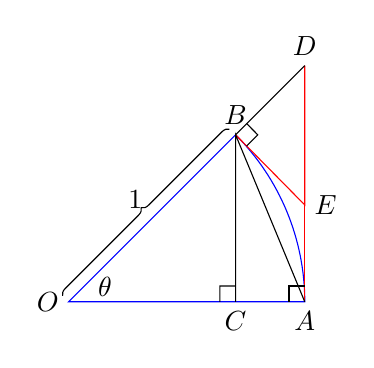
\begin{tikzpicture}[scale=3]
\coordinate (O) at (0,0);
\coordinate (A) at (1,0);
\coordinate (B) at (45:1);
\coordinate (C) at (B |- 0,0);
\coordinate (D) at (1,1);
\coordinate (E) at (1,0.41);
\draw[blue] (O) -- (A) arc [start angle=0, end angle=45, radius=1] -- cycle;
\draw[red] (A) -- (E);
\draw[red] (B) -- (E) -- (D);
\draw[black] (B) -- (D);
\draw[black] (A) -- (B) -- (C);
\node[left] at (O) {$O$};
\node[below] at (A) {$A$};
\node[above] at (B) {$B$};
\node[below] at (C) {$C$};
\node[above] at (D) {$D$};
\node[right] at (E) {$E$};
\draw[decoration={brace,raise=3pt},decorate] (0,0) -- (45:1) node[pos=0.5, above left]{$1$};
\draw pic["$\theta$",-,angle eccentricity=1, angle radius=0.5cm]{angle=A--O--B};
\draw pic[draw,-,angle eccentricity=1.4, angle radius=0.2cm]{right angle=B--C--O};
\draw pic[draw,-,angle eccentricity=1.4, angle radius=0.2cm]{right angle=E--B--D};
\draw pic[draw,-,angle eccentricity=1.4, angle radius=0.2cm]{right angle=D--A--O};
\end{tikzpicture}
\end{center}

\newpage

This is a limit problem from Stewart: (credit for first diagram: Stewart, second diagram with auxillary aid is mine)

\begin{center}
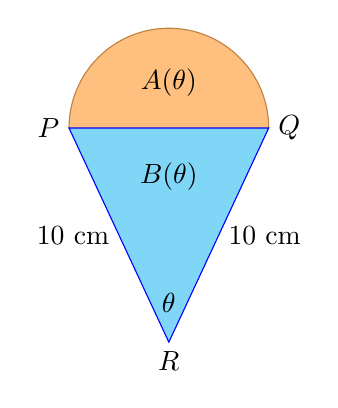
\begin{tikzpicture}[scale=3]
\coordinate (P) at (115:1);
\coordinate (Q) at (65:1);
\coordinate (R) at (0,0);
\path[fill=orange,opacity=0.5] (Q) arc [start angle=0, end angle=180, radius=0.4226] -- cycle;
\draw[brown] (Q) arc [start angle=0, end angle=180, radius=0.4226];
\path[fill=cyan,opacity=0.5] (P) -- (Q) -- (R) -- cycle;
\draw[blue] (P) -- (Q) -- node[right]{{\color{black}10 cm}} (R) -- node[left]{{\color{black}10 cm}} cycle;
\node[left] at (P) {$P$};
\node[right] at (Q) {$Q$};
\node[below] at (R) {$R$};
\draw pic["$\theta$",-,angle eccentricity=1, angle radius=0.5cm]{angle=Q--R--P};
\node at (0,1.1) {$A(\theta)$};
\node at (0,0.7) {$B(\theta)$};
\end{tikzpicture}
\hspace{20pt}
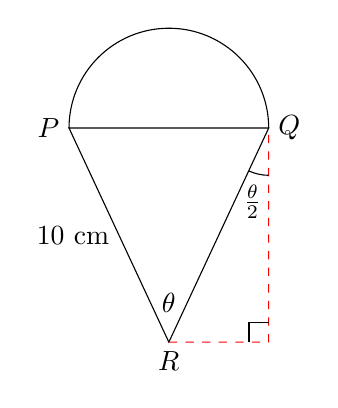
\begin{tikzpicture}[scale=3]
\coordinate (P) at (115:1);
\coordinate (Q) at (65:1);
\coordinate (R) at (0,0);
\draw (Q) arc [start angle=0, end angle=180, radius=0.4226];
\draw (P) -- (Q) -- (R) -- node[left]{{\color{black}10 cm}} cycle;
\node[left] at (P) {$P$};
\node[right] at (Q) {$Q$};
\node[below] at (R) {$R$};
\draw pic["$\theta$",-,angle eccentricity=1, angle radius=0.5cm]{angle=Q--R--P};
\coordinate (AUX) at (Q |- 0,0);
\draw[red,dashed] (R) -- (AUX) -- (Q); 
\draw pic["$\frac{\theta}{2}$",-,angle eccentricity=1.6, angle radius=0.6cm,draw]{angle=R--Q--AUX};
\draw pic["",-,angle eccentricity=1.6, angle radius=0.25cm,draw]{right angle=Q--AUX--R};
\end{tikzpicture}
\end{center}

And this is a trigonometric function: (based on diagram from Stewart)

\begin{center}
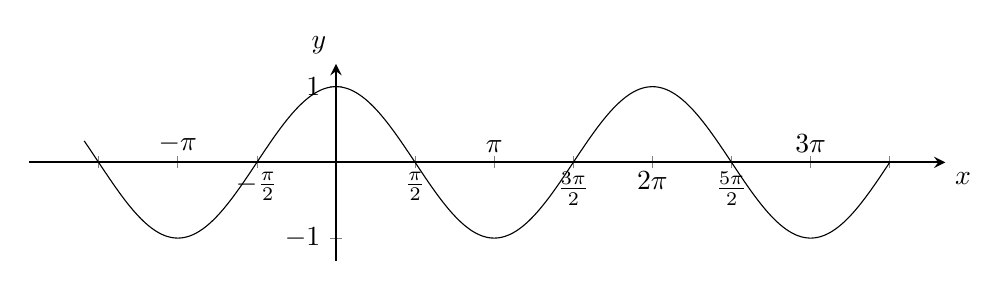
\begin{tikzpicture}
\begin{axis}[
standard,
xmin=-4, xmax=10,
xtick={-3.14159*3/2,-3.14159,-3.14159/2,3.14159/2,3.14159,3.14159*3/2,3.14159*2,3.14159*5/2,3.14159*3,3.14159*7/2}, ytick={-1,1},
xticklabels={}, yticklabels={$-1$,$1$},
xlabel={$x$}, ylabel={$y$},
  width=.96\linewidth,
    height=2.5cm,
    scale only axis=true]
\addplot[domain=-5:11,samples=300] {cos(deg(x))};
\node[above] at (-3.14159,0) {$-\pi$};
\node[above] at (3.14159,0) {$\pi$};
\node[above] at (3.14159*3,0) {$3\pi$};
\node[below] at (-3.14159/2,0) {$-\frac{\pi}{2}$};
\node[below] at (3.14159/2,0) {$\frac{\pi}{2}$};
\node[below] at (3.14159*3/2,0) {$\frac{3\pi}{2}$};
\node[below] at (3.14159*2,0) {$2\pi$};
\node[below] at (3.14159*5/2,0) {$\frac{5\pi}{2}$};
\end{axis}
\end{tikzpicture}
\end{center}

And I am capable of much more! As an example, I can make beautiful volumes of revolution diagrams, but didn't include any since they were lost in a computer backup and I'm too tired to make any now.

\end{document}